%  Pt2.tex
% !TeX spellcheck = en_GB
% !TeX root = ProjectRiskManagement.tex

\section{Identify all relevant sources of uncertainty} \label{s:Identify}
%\todo{900 Words}

% the identify phase of the PUMP approach, in the execution and delivery strategy shaping phase of a project’s lifecycle, explain concisely in your own words what you believe are the key features of a PUMP approach, comparing these features with the PMI PIMBOK approach or any other form of common practice you are familiar with. Your discussion should demonstrate your ability to understand a particular area of the course material in depth, based on selective reading, critical analysis and the case study exercise. Use examples to illustrate your discussion if you wish, making use of the Samdo case study if you wish, but concentrate on concepts and principles. Build on your Part 1 answer, avoiding repetition of earlier discussion.
%900words.

%Key Features

%Compare with PMI PMBOK or others

%In depth understanding

The identify phase is commonplace in several risk management methodologies, including PUMPs. 
However, there is a marked removal from best practice in the PUMP approach resulting in an iterative, holistic, inherently creative method to identify all relevant sources of uncertainty, possible response options, assumptions, conditions and second-order sources.
This encourages the consideration of all types of uncertainty to a relevant degree of detail thus achieving clarity efficiency.

The common practice approach is a linear process whereby all relevant risk events must be identified at an early stage. 
The response identification or formulation of mitigation strategies is left until later in the linear process and decoupled from the identification of the sources themselves.
Assumptions and conditions are also decoupled, since unbiased estimation is not a formal goal of the process. 
This approach does not offer optimum clarity efficiency, since decoupled consideration is much more difficult to address.
Moreover, a dangerous false sense of security can be created through best practice approaches where linearity obscures the underlying complexity which may ultimately endanger the achievement of project objectives.
                         
Within the PUMP framework, the identification of sources of uncertainty and possible response options are closely coupled. 
Considering response options as new sources are identified increases the chances of developing powerful general responses that are crucial to deliver clarity efficiency. 
Moreover, unidentified responses contribute to ambiguity uncertainty. 
On some occasions the consequences of the response can lead to secondary sources which may also require consideration.
The identify phase allows an enlightened reshaping of relevant base plans and contingency plans as required.

\begin{figure}[!h]
  \centering
    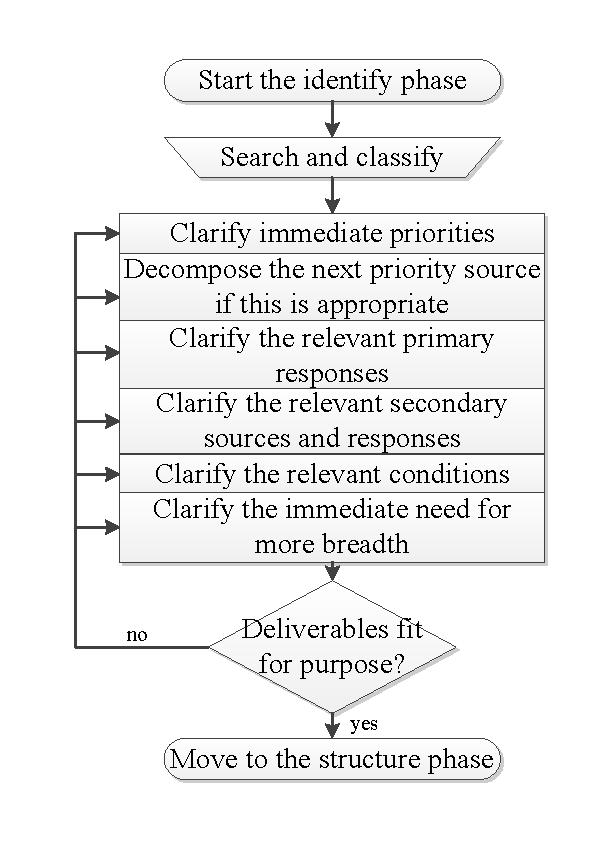
\includegraphics[width = 0.5\textwidth]{./Figures/Identify.pdf} 
\caption{Identify Phase Process - adapted from \cite{chapman}}
\label{Figure:Identify}
\end{figure}

The process has two main features. 
The \textbf{search} task involves finding all relevant sources responses and conditions. 
The \textbf{classify} task provides a suitable structure where sources have been aggregated or decomposed as necessary upon which further analysis can proceed.
The process is shown in figure \ref{Figure:Identify}.
The keyword in the process is `relevant'. 
The skill of the risk practitioner is in seeing where maintaining strategic level composite sources or decomposing to further levels of detail is strategically helpful.



\inote{Identification of responses}
\inote{Embracing and encouraging creativity}

\begin{figure}[!h]
  \centering
    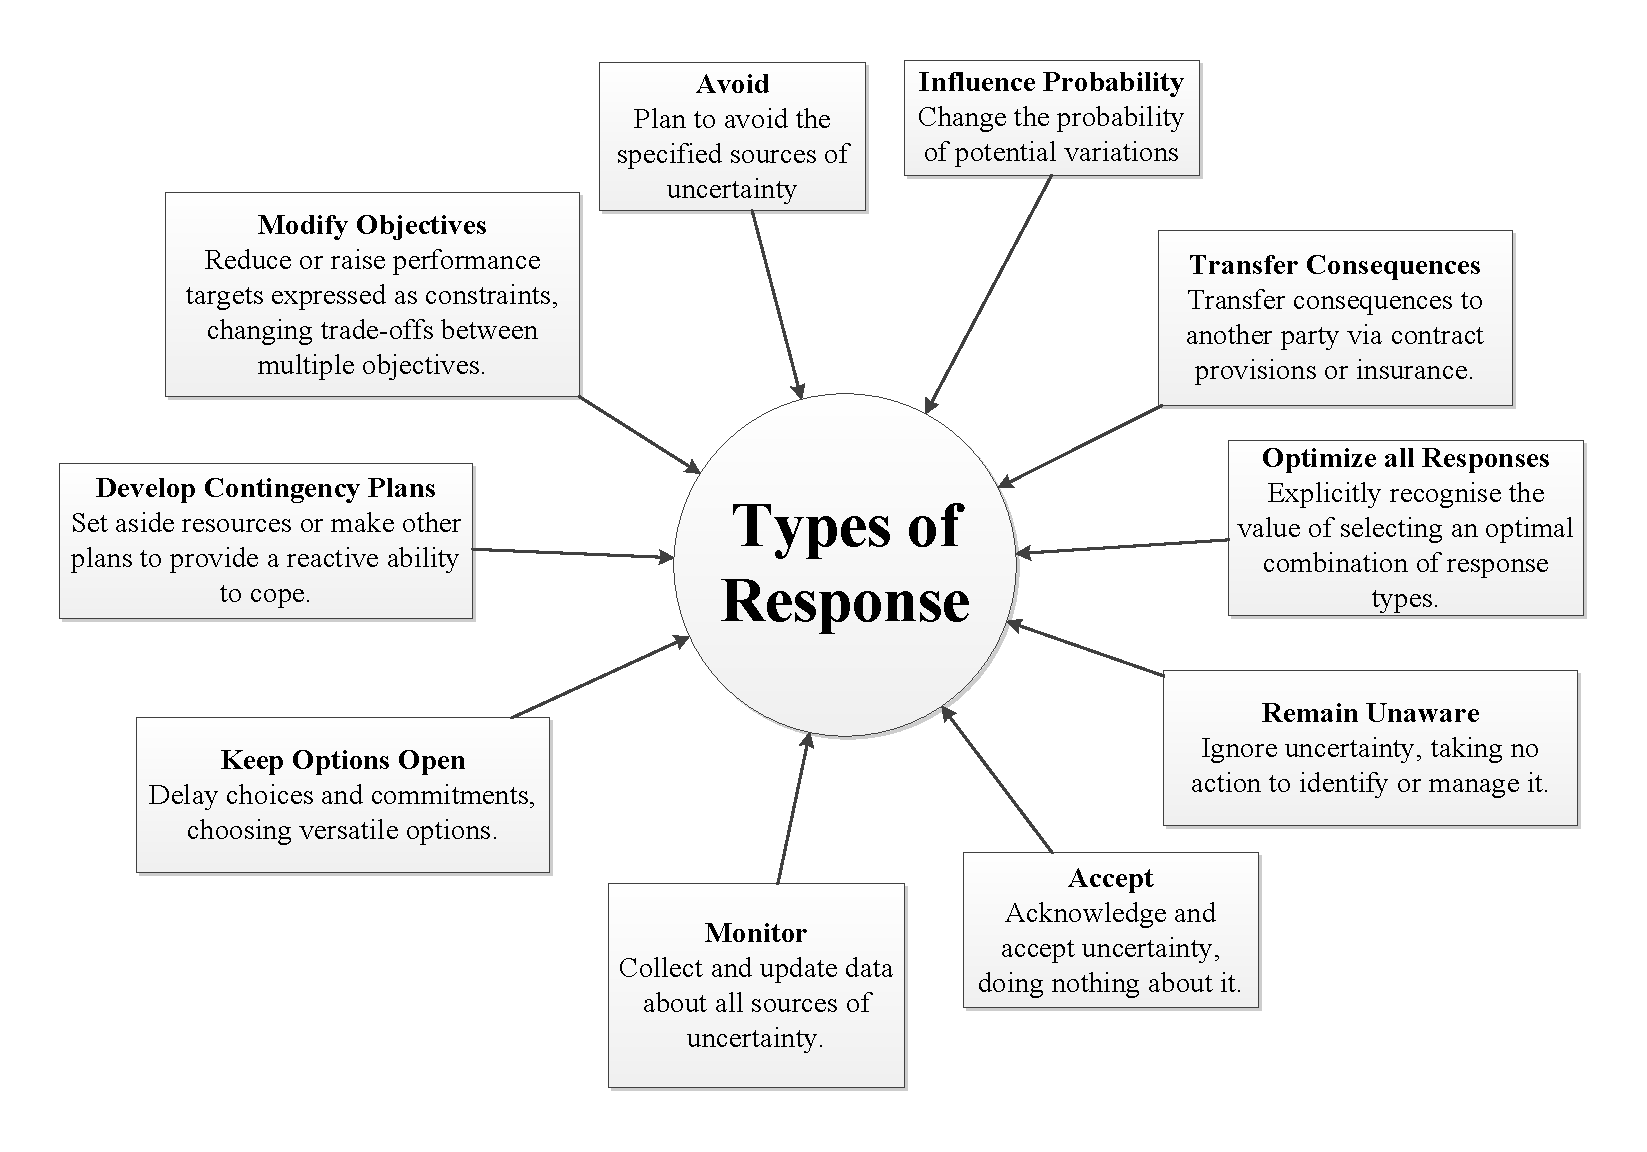
\includegraphics[width = \textwidth]{./Figures/ResponseTypes.pdf} 
\caption{Generic response types - adapted from \cite{chapman}}
\label{Figure:Identify}
\end{figure}

\inote{Conclusions}








